%% Standalone lecture -- build with:  pdflatex -shell-escape wasserstein
%% Shared preamble for standalone lecture files.
%%
%% Every lecture begins with %% Shared preamble for standalone lecture files.
%%
%% Every lecture begins with %% Shared preamble for standalone lecture files.
%%
%% Every lecture begins with \input{preamble} and is compiled on its own:
%%     pdflatex -shell-escape <lecture>
%% There is no master lectures.tex any more -- the list of lectures lives in
%% lectures.yaml and is read by the build scripts.

\documentclass[25pt,landscape,footrule]{foils}
\input{macros_gen}
\backgroundsetup{contents={}}

\usepackage{stmaryrd}
\usepackage{ifthen}
\usepackage{pdf14}

% Every figure lives in this course's lectures/figures (consolidated
% 2026-10-08).  Do not add other courses' folders back: when a name exists in
% several folders LaTeX silently takes the first, which mixed old and new
% frames of the same animation.  A missing figure should be a build error.
\graphicspath{{figures/}{../lectures/figures/}}

\date{}

\newcounter{lessoncnt}
\newcommand{\lesson}[1]{\setcounter{page}{1}%
\section{Mathematics of Machine Learning\\%
\vfill
\textcolor{red}{\textit{#1}}
\vfill}}
 and is compiled on its own:
%%     pdflatex -shell-escape <lecture>
%% There is no master lectures.tex any more -- the list of lectures lives in
%% lectures.yaml and is read by the build scripts.

\documentclass[25pt,landscape,footrule]{foils}
%\usepackage[compat2,pdftex]{geometry}
\usepackage[pdftex]{geometry}
\geometry{headsep=-2.5ex,hscale=0.9,bmargin=2.5cm,tmargin=1cm,textwidth=25cm}
\usepackage[pdftex]{xcolor}
\usepackage{pause}
\usepackage{background}
%\usepackage[color=white]{background}
\usepackage{listings}
\usepackage{graphicx}
\usepackage{epsfig}
\usepackage{epstopdf}
\usepackage{bm}
\usepackage{amssymb}
\usepackage{amsfonts}
\usepackage{marvosym}
\usepackage{cite}
\usepackage{pifont}
\usepackage[english]{babel}
\usepackage{amsmath}
\usepackage{amsfonts}
\usepackage{rotating}
\usepackage{listings}
\usepackage{pp4slide}
%\usepackage{hyperref}
\usepackage{pp4link}
\usepackage{fancyvrb}
\usepackage{multido}
\usepackage{calc}
\usepackage{mleftright}
\mleftright % Redefines \left to \mleft and \right to \mright



\thinmuskip=1mu

\newcommand{\bigstrut}{\rule[-0.5\baselineskip]{0pt}{1.2\baselineskip}}
\renewcommand{\ttdefault}{pcr}

\newcommand{\squeeze}{\setlength{\itemsep}{-2pt}}
%\renewcommand{\familydefault}{cmr}
%\renewcommand{\labelitemii}{\textcolor{green}{$\star$}}
\newcommand{\tick}{{\large \ding{51}}}
\newcommand{\cross}{{\large \ding{55}}}
%\DeclareMathAlphabet{\mat}{OT1}{cmss}{bx}{n}
\DeclareMathAlphabet{\mat}{U}{eur}{b}{n}
\newcommand{\figs}{/home/apb/figures}
\newcommand{\stimes}{{\scriptstyle \times}}
\newcommand{\tr}{\textsf{T}}
\newcommand{\e}[1]{{\rm e}^{#1}}
\newcommand{\E}[1]{{\rm e}^{{\displaystyle #1}}}
\newcommand{\av}[2][]{\mathbb{E}_{#1}\left[ #2 \right]}
\newcommand{\Var}[1]{\mathbb{V}\mathrm{ar}\left( #1 \right)}
\newcommand{\pred}[1]{\left\llbracket { \small #1} \right\rrbracket}
\newcommand{\logg}[1]{\log\left( #1 \right)}
\newcommand{\logtwo}[1]{\log_2\left( #1 \right)}
\newcommand{\bra}[1]{\left( #1 \right)}
\newcommand{\prob}[1]{\mathbb{P}\left( #1 \right)}
\newcommand{\Prob}[1]{\mathbb{P}\left( #1 \right)}
\newcommand{\Step}{\mathop{\mat{\Theta}}}
\newcommand\diag{\mathop{\mathrm{diag}}}
\newcommand{\grad}{\bm{\nabla}}
\newcommand{\gradx}{\bm{\nabla}_{\!\!\scriptscriptstyle \bm{x}}}
\newcommand{\gradw}{\bm{\nabla}_{\!\!\scriptscriptstyle \bm{w}}}
\newcommand{\dd}{\mathrm{d}}
\newcommand{\ii}{\mathrm{i}}
\newcommand{\data}{\mathcal{D}}
\newcommand{\class}{\mathcal{C}}
\newcommand{\hypo}{\mathcal{H}}
\newcommand{\indep}{\perp \!\!\!\! \perp}
\newcommand{\pd}[3][\,]{\frac{\partial^{#1}{#2}}{\partial\,{#3}}}
\newcommand{\normal}[1]{\mathcal{N}\!\left( #1 \right)}
\newcommand{\Dist}[2][Binom]{\mathrm{#1}\left( \strut {#2} \right)}
\newcommand{\brackets}[1]{\!\left( #1 \right)}
\newcommand{\KL}[2]{\mathop{\mathrm{KL}}\left(#1 \big\| #2\right)}
\newcommand{\argmax}{\mathop{\mathrm{argmax}}}
\newcommand{\argmin}{\mathop{\mathrm{argmin}}}
\newcommand{\margin}{\Delta}
\lstnewenvironment{matlab}[1][frame=TB]{\lstset{#1}}{}       
%\renewcommand{\emph}[1]{\textcolor{red}{\textbf{#1}}}
\newcommand{\myskip}[1]{}
\newcommand\mycom[2]{\genfrac{}{}{0pt}{}{#1}{#2}}
\newcommand{\jl}{\lstinline[basicstyle=\ttfamily\color{DarkGreen},%
 keywordstyle=\bfseries\ttfamily\color{DarkGreen}]}
\definecolor{EmphColor}{rgb}{0.0,0.0,1.0}
\renewcommand{\emph}[1]{{\color{EmphColor}\textbf{#1}}}
\newcommand{\len}[1]{\| #1 \|}
\newcommand{\inner}[2]{\left\langle {#1}, {#2}\right\rangle}
\newenvironment{psmallmatrix}{\left(\begin{smallmatrix}}{\end{smallmatrix}\right)}
  

\definecolor{DarkGreen}{rgb}{0,0.5,0}
\definecolor{DarkRed}{rgb}{0,0,0.5}
\definecolor{HighLight}{rgb}{1,0,0}     % yellow
\definecolor{TextColor}{rgb}{0.0,0.1,0.1}     % white
\definecolor{TwoColor}{rgb}{0.0,0.5,0.1}      % used for switching colors

\definecolor{HeadLineColor}{rgb}{1.0,0.0,0.0} % cyan
\definecolor{SpecialColor}{rgb}{0.53,0.81,1.0}
\renewcommand{\normalcolor}{\color{HeadLineColor}}

\pausecolors{TwoColor}{TextColor}{HighLight}
\pausecolors{EmphColor}{TextColor}{EmphColor}
\pausecolors{DarkGreen}{DarkGreen}{DarkRed}
\pausecolors{SpecialColor}{white}{HighLight}

\newenvironment{PauseHighLight}{\color{TwoColor}\pausehighlight}{}
\newcommand{\multipdf}[2][width=\linewidth]{\multiinclude[pause=\pauselevel{:+0}\pause,format=pdf,graphics={#1}]{#2}}

\lstdefinelanguage{pseudo}
 {keywords={all,and,begin,break,continue,do,else,elseif,%
     end,endif,endfor,endwhile,%
     exit,false,for,forall,goto,if,%
     or,return,then,true,to,repeat,until,while},%
  comment=[s]{/*}{*/},%
  morecomment=[l]//,%
  morestring=[d]"%
 }[keywords,comments,strings]


\lstloadlanguages{Java,pseudo,Python}
\lstset{
  basicstyle=\footnotesize\ttfamily\color{DarkGreen},
  keywordstyle=\bfseries\footnotesize\ttfamily\color{DarkGreen},
  commentstyle=\footnotesize\it\rmfamily\color{blue},
  language=Java,
  showstringspaces=false
  }


\lstnewenvironment{pseudo}[1][]{\lstset{language=pseudo,mathescape,literate={:=}{{$\gets$}}2 {!}{{$\neg$}}1 {!=}{{\!\!$\neq$\,\,}}2 {<=}{{\!\!$\leq$\,\,}}2 {>=}{{\!\!$\geq$\,\,}}2,escapechar=\#,#1}}{}
\lstnewenvironment{java}[1][]{\lstset{escapechar=\$,#1}}{}
% Python code: the language setting makes # comments use commentstyle.
% Comments stay monospaced: the default italic roman letter-spaces badly
% on listings' fixed columns.
\lstnewenvironment{python}[1][frame=TB]{\lstset{language=Python,
    commentstyle=\footnotesize\ttfamily\color{blue},#1}}{}

\MyLogo{}
%\Restriction{}
%\rightfooter{\hyperlink{overview}{$\square$}}

\newcommand{\keywords}[1]{\vfill{\noindent\it #1}}

\newcounter{outlineitem}
\setcounter{outlineitem}{0}
\newcommand{\outlineitem}[2]{\item%
  \def\targ{\value{emumi}}%
  \ifnum\value{enumi}=\value{outlineitem}%
  \color{HighLight}\textbf{#1}\toptarget{#2}\color{TextColor}%
   \else\toplink{#2}{#1}\fi
}
\color{TwoColor}


%-- Instead of writing \section we want the file structured by \section.
\newcommand{\section}[2][0]{\foilhead[#1cm]{#2}}

%-- Write each page into a \begin{slide} -- \end{slide} environment.
\newenvironment{slide}{}{\pauselevel{=1}}

\MyLogo{\pauselevel{=1}\Acrobatmenu{GoBack}{%
  \color{TextColor}{Adam Pr\"ugel-Bennett}} \hspace{2cm}
  % Clicking on the name steps one slide back.
  \toplink{firstoutline}{\color{red}Mathematics of Machine
    Learning}%
  \hspace{2cm}
  \texttt{//ecs-vlc.github.io/aice3001/}
  %Clicking on the date jumps to the last page, which should be the
  %table of contents.
  \rightfooter{\Acrobatmenu{LastPage}{\qquad%
  \textsf{\color{TextColor}\tiny\thepage}}}% page number
  % Clicking on the page number steps one slide back.
}
\raggedright
\newcommand{\Outline}{}

\newcommand{\pb}{\pausebuild \color{TwoColor}}
\newcommand{\pauseb}{\pauselevel{build, highlight}\pause}
\newcommand{\hl}[1]{\pauselevel{=1, highlight =1 :1, highlight =#1 :#1}\pause}
\newcommand{\hll}{\pauselevel{=1, highlight =1 :1}\pause}
\newcommand{\pauseh}{\pauselevel{highlight}\pause}
\newcommand{\nhl}[1]{\textcolor{TextColor}{#1}}
\newcommand{\mypl}[1]{\pauselevel{=#1 :#1}\pause}
\input supp-pdf.tex
\DeclareGraphicsRule{*}{mps}{*}{}
\usepackage{mpmulti}
%\leftheader{}
\rightheader{} % no more page numbers on top right


\hypersetup{pdftitle={ECS Lectures},pdfsubject={Machine Learning}
pdfauthor={Adam Prugel-Bennett},pdfkeywords={machine learning},
pdfpagemode={FullScreen},
bookmarksopen=false,
hypertexnames=false,pdfstartview={FitV},colorlinks,linkcolor={blue},
citecolor={green},urlcolor={blue}}



\newcommand\bluepage{
\clearpage
\renewcommand\normalcolor{\color{yellow}}
\pagecolor{blue}
\renewcommand\Black{\color{white}}
\color{white}
\hypersetup{colorlinks=true}
}

\newcommand\whitepage{
\clearpage
\renewcommand\normalcolor{\color{black}}
\pagecolor{white}
\renewcommand\Black{\color{black}}
\color{black}
\hypersetup{colorlinks=true}
}

\whitepage
\setlength{\unitlength}{1mm}

\newenvironment{leftImage}[2][0.3]{%
\begin{minipage}{#1\linewidth}
  \includegraphics[width=\linewidth]{#2}
\end{minipage}\hfill
\begin{minipage}{0.92\linewidth - #1\linewidth}}%
{\end{minipage}}

\newenvironment{rightImage}[2][0.3]{%
\newcommand{\foot}{\begin{minipage}{#1\linewidth}\includegraphics[width=0.98\linewidth]{#2}\end{minipage}}%
\begin{minipage}{0.95\linewidth - #1\linewidth}\raggedright }{\end{minipage}\hfill\foot}


%%% Local Variables: 
%%% mode: latex
%%% TeX-master: t
%%% End: 

\backgroundsetup{contents={}}

\usepackage{stmaryrd}
\usepackage{ifthen}
\usepackage{pdf14}

% Every figure lives in this course's lectures/figures (consolidated
% 2026-10-08).  Do not add other courses' folders back: when a name exists in
% several folders LaTeX silently takes the first, which mixed old and new
% frames of the same animation.  A missing figure should be a build error.
\graphicspath{{figures/}{../lectures/figures/}}

\date{}

\newcounter{lessoncnt}
\newcommand{\lesson}[1]{\setcounter{page}{1}%
\section{Mathematics of Machine Learning\\%
\vfill
\textcolor{red}{\textit{#1}}
\vfill}}
 and is compiled on its own:
%%     pdflatex -shell-escape <lecture>
%% There is no master lectures.tex any more -- the list of lectures lives in
%% lectures.yaml and is read by the build scripts.

\documentclass[25pt,landscape,footrule]{foils}
%\usepackage[compat2,pdftex]{geometry}
\usepackage[pdftex]{geometry}
\geometry{headsep=-2.5ex,hscale=0.9,bmargin=2.5cm,tmargin=1cm,textwidth=25cm}
\usepackage[pdftex]{xcolor}
\usepackage{pause}
\usepackage{background}
%\usepackage[color=white]{background}
\usepackage{listings}
\usepackage{graphicx}
\usepackage{epsfig}
\usepackage{epstopdf}
\usepackage{bm}
\usepackage{amssymb}
\usepackage{amsfonts}
\usepackage{marvosym}
\usepackage{cite}
\usepackage{pifont}
\usepackage[english]{babel}
\usepackage{amsmath}
\usepackage{amsfonts}
\usepackage{rotating}
\usepackage{listings}
\usepackage{pp4slide}
%\usepackage{hyperref}
\usepackage{pp4link}
\usepackage{fancyvrb}
\usepackage{multido}
\usepackage{calc}
\usepackage{mleftright}
\mleftright % Redefines \left to \mleft and \right to \mright



\thinmuskip=1mu

\newcommand{\bigstrut}{\rule[-0.5\baselineskip]{0pt}{1.2\baselineskip}}
\renewcommand{\ttdefault}{pcr}

\newcommand{\squeeze}{\setlength{\itemsep}{-2pt}}
%\renewcommand{\familydefault}{cmr}
%\renewcommand{\labelitemii}{\textcolor{green}{$\star$}}
\newcommand{\tick}{{\large \ding{51}}}
\newcommand{\cross}{{\large \ding{55}}}
%\DeclareMathAlphabet{\mat}{OT1}{cmss}{bx}{n}
\DeclareMathAlphabet{\mat}{U}{eur}{b}{n}
\newcommand{\figs}{/home/apb/figures}
\newcommand{\stimes}{{\scriptstyle \times}}
\newcommand{\tr}{\textsf{T}}
\newcommand{\e}[1]{{\rm e}^{#1}}
\newcommand{\E}[1]{{\rm e}^{{\displaystyle #1}}}
\newcommand{\av}[2][]{\mathbb{E}_{#1}\left[ #2 \right]}
\newcommand{\Var}[1]{\mathbb{V}\mathrm{ar}\left( #1 \right)}
\newcommand{\pred}[1]{\left\llbracket { \small #1} \right\rrbracket}
\newcommand{\logg}[1]{\log\left( #1 \right)}
\newcommand{\logtwo}[1]{\log_2\left( #1 \right)}
\newcommand{\bra}[1]{\left( #1 \right)}
\newcommand{\prob}[1]{\mathbb{P}\left( #1 \right)}
\newcommand{\Prob}[1]{\mathbb{P}\left( #1 \right)}
\newcommand{\Step}{\mathop{\mat{\Theta}}}
\newcommand\diag{\mathop{\mathrm{diag}}}
\newcommand{\grad}{\bm{\nabla}}
\newcommand{\gradx}{\bm{\nabla}_{\!\!\scriptscriptstyle \bm{x}}}
\newcommand{\gradw}{\bm{\nabla}_{\!\!\scriptscriptstyle \bm{w}}}
\newcommand{\dd}{\mathrm{d}}
\newcommand{\ii}{\mathrm{i}}
\newcommand{\data}{\mathcal{D}}
\newcommand{\class}{\mathcal{C}}
\newcommand{\hypo}{\mathcal{H}}
\newcommand{\indep}{\perp \!\!\!\! \perp}
\newcommand{\pd}[3][\,]{\frac{\partial^{#1}{#2}}{\partial\,{#3}}}
\newcommand{\normal}[1]{\mathcal{N}\!\left( #1 \right)}
\newcommand{\Dist}[2][Binom]{\mathrm{#1}\left( \strut {#2} \right)}
\newcommand{\brackets}[1]{\!\left( #1 \right)}
\newcommand{\KL}[2]{\mathop{\mathrm{KL}}\left(#1 \big\| #2\right)}
\newcommand{\argmax}{\mathop{\mathrm{argmax}}}
\newcommand{\argmin}{\mathop{\mathrm{argmin}}}
\newcommand{\margin}{\Delta}
\lstnewenvironment{matlab}[1][frame=TB]{\lstset{#1}}{}       
%\renewcommand{\emph}[1]{\textcolor{red}{\textbf{#1}}}
\newcommand{\myskip}[1]{}
\newcommand\mycom[2]{\genfrac{}{}{0pt}{}{#1}{#2}}
\newcommand{\jl}{\lstinline[basicstyle=\ttfamily\color{DarkGreen},%
 keywordstyle=\bfseries\ttfamily\color{DarkGreen}]}
\definecolor{EmphColor}{rgb}{0.0,0.0,1.0}
\renewcommand{\emph}[1]{{\color{EmphColor}\textbf{#1}}}
\newcommand{\len}[1]{\| #1 \|}
\newcommand{\inner}[2]{\left\langle {#1}, {#2}\right\rangle}
\newenvironment{psmallmatrix}{\left(\begin{smallmatrix}}{\end{smallmatrix}\right)}
  

\definecolor{DarkGreen}{rgb}{0,0.5,0}
\definecolor{DarkRed}{rgb}{0,0,0.5}
\definecolor{HighLight}{rgb}{1,0,0}     % yellow
\definecolor{TextColor}{rgb}{0.0,0.1,0.1}     % white
\definecolor{TwoColor}{rgb}{0.0,0.5,0.1}      % used for switching colors

\definecolor{HeadLineColor}{rgb}{1.0,0.0,0.0} % cyan
\definecolor{SpecialColor}{rgb}{0.53,0.81,1.0}
\renewcommand{\normalcolor}{\color{HeadLineColor}}

\pausecolors{TwoColor}{TextColor}{HighLight}
\pausecolors{EmphColor}{TextColor}{EmphColor}
\pausecolors{DarkGreen}{DarkGreen}{DarkRed}
\pausecolors{SpecialColor}{white}{HighLight}

\newenvironment{PauseHighLight}{\color{TwoColor}\pausehighlight}{}
\newcommand{\multipdf}[2][width=\linewidth]{\multiinclude[pause=\pauselevel{:+0}\pause,format=pdf,graphics={#1}]{#2}}

\lstdefinelanguage{pseudo}
 {keywords={all,and,begin,break,continue,do,else,elseif,%
     end,endif,endfor,endwhile,%
     exit,false,for,forall,goto,if,%
     or,return,then,true,to,repeat,until,while},%
  comment=[s]{/*}{*/},%
  morecomment=[l]//,%
  morestring=[d]"%
 }[keywords,comments,strings]


\lstloadlanguages{Java,pseudo,Python}
\lstset{
  basicstyle=\footnotesize\ttfamily\color{DarkGreen},
  keywordstyle=\bfseries\footnotesize\ttfamily\color{DarkGreen},
  commentstyle=\footnotesize\it\rmfamily\color{blue},
  language=Java,
  showstringspaces=false
  }


\lstnewenvironment{pseudo}[1][]{\lstset{language=pseudo,mathescape,literate={:=}{{$\gets$}}2 {!}{{$\neg$}}1 {!=}{{\!\!$\neq$\,\,}}2 {<=}{{\!\!$\leq$\,\,}}2 {>=}{{\!\!$\geq$\,\,}}2,escapechar=\#,#1}}{}
\lstnewenvironment{java}[1][]{\lstset{escapechar=\$,#1}}{}
% Python code: the language setting makes # comments use commentstyle.
% Comments stay monospaced: the default italic roman letter-spaces badly
% on listings' fixed columns.
\lstnewenvironment{python}[1][frame=TB]{\lstset{language=Python,
    commentstyle=\footnotesize\ttfamily\color{blue},#1}}{}

\MyLogo{}
%\Restriction{}
%\rightfooter{\hyperlink{overview}{$\square$}}

\newcommand{\keywords}[1]{\vfill{\noindent\it #1}}

\newcounter{outlineitem}
\setcounter{outlineitem}{0}
\newcommand{\outlineitem}[2]{\item%
  \def\targ{\value{emumi}}%
  \ifnum\value{enumi}=\value{outlineitem}%
  \color{HighLight}\textbf{#1}\toptarget{#2}\color{TextColor}%
   \else\toplink{#2}{#1}\fi
}
\color{TwoColor}


%-- Instead of writing \section we want the file structured by \section.
\newcommand{\section}[2][0]{\foilhead[#1cm]{#2}}

%-- Write each page into a \begin{slide} -- \end{slide} environment.
\newenvironment{slide}{}{\pauselevel{=1}}

\MyLogo{\pauselevel{=1}\Acrobatmenu{GoBack}{%
  \color{TextColor}{Adam Pr\"ugel-Bennett}} \hspace{2cm}
  % Clicking on the name steps one slide back.
  \toplink{firstoutline}{\color{red}Mathematics of Machine
    Learning}%
  \hspace{2cm}
  \texttt{//ecs-vlc.github.io/aice3001/}
  %Clicking on the date jumps to the last page, which should be the
  %table of contents.
  \rightfooter{\Acrobatmenu{LastPage}{\qquad%
  \textsf{\color{TextColor}\tiny\thepage}}}% page number
  % Clicking on the page number steps one slide back.
}
\raggedright
\newcommand{\Outline}{}

\newcommand{\pb}{\pausebuild \color{TwoColor}}
\newcommand{\pauseb}{\pauselevel{build, highlight}\pause}
\newcommand{\hl}[1]{\pauselevel{=1, highlight =1 :1, highlight =#1 :#1}\pause}
\newcommand{\hll}{\pauselevel{=1, highlight =1 :1}\pause}
\newcommand{\pauseh}{\pauselevel{highlight}\pause}
\newcommand{\nhl}[1]{\textcolor{TextColor}{#1}}
\newcommand{\mypl}[1]{\pauselevel{=#1 :#1}\pause}
\input supp-pdf.tex
\DeclareGraphicsRule{*}{mps}{*}{}
\usepackage{mpmulti}
%\leftheader{}
\rightheader{} % no more page numbers on top right


\hypersetup{pdftitle={ECS Lectures},pdfsubject={Machine Learning}
pdfauthor={Adam Prugel-Bennett},pdfkeywords={machine learning},
pdfpagemode={FullScreen},
bookmarksopen=false,
hypertexnames=false,pdfstartview={FitV},colorlinks,linkcolor={blue},
citecolor={green},urlcolor={blue}}



\newcommand\bluepage{
\clearpage
\renewcommand\normalcolor{\color{yellow}}
\pagecolor{blue}
\renewcommand\Black{\color{white}}
\color{white}
\hypersetup{colorlinks=true}
}

\newcommand\whitepage{
\clearpage
\renewcommand\normalcolor{\color{black}}
\pagecolor{white}
\renewcommand\Black{\color{black}}
\color{black}
\hypersetup{colorlinks=true}
}

\whitepage
\setlength{\unitlength}{1mm}

\newenvironment{leftImage}[2][0.3]{%
\begin{minipage}{#1\linewidth}
  \includegraphics[width=\linewidth]{#2}
\end{minipage}\hfill
\begin{minipage}{0.92\linewidth - #1\linewidth}}%
{\end{minipage}}

\newenvironment{rightImage}[2][0.3]{%
\newcommand{\foot}{\begin{minipage}{#1\linewidth}\includegraphics[width=0.98\linewidth]{#2}\end{minipage}}%
\begin{minipage}{0.95\linewidth - #1\linewidth}\raggedright }{\end{minipage}\hfill\foot}


%%% Local Variables: 
%%% mode: latex
%%% TeX-master: t
%%% End: 

\backgroundsetup{contents={}}

\usepackage{stmaryrd}
\usepackage{ifthen}
\usepackage{pdf14}

% Every figure lives in this course's lectures/figures (consolidated
% 2026-10-08).  Do not add other courses' folders back: when a name exists in
% several folders LaTeX silently takes the first, which mixed old and new
% frames of the same animation.  A missing figure should be a build error.
\graphicspath{{figures/}{../lectures/figures/}}

\date{}

\newcounter{lessoncnt}
\newcommand{\lesson}[1]{\setcounter{page}{1}%
\section{Mathematics of Machine Learning\\%
\vfill
\textcolor{red}{\textit{#1}}
\vfill}}


\begin{document}

\lesson{Optimal Transport and the Wasserstein Distance}
\vspace{-1cm}
\begin{center}
  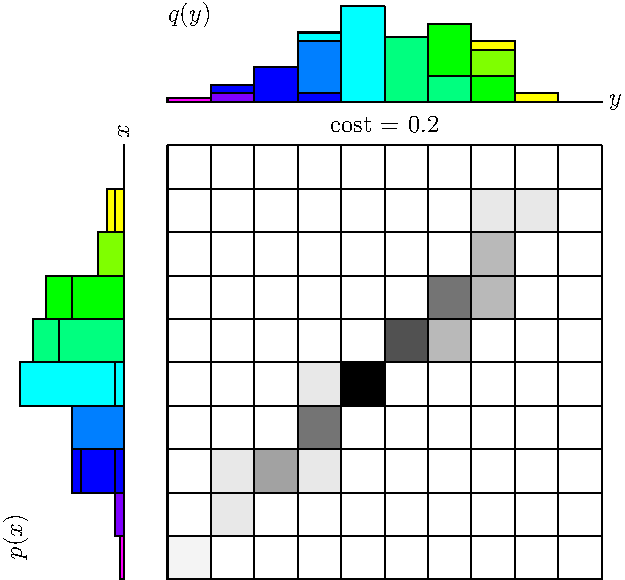
\includegraphics[width=0.38\linewidth]{transportationCost-5}
\end{center}

\keywords{Wasserstein distance, optimal transport, duality, Lipschitz functions, WGANs, Sinkhorn, FID}


%%%%%%%%%%%%%%%%%%%%%%% Next Slide %%%%%%%%%%%%%%%%%%%%%%%
\renewcommand{\Outline}{%
\begin{slide}
\section{Outline}

\begin{minipage}{9cm}\raggedright
  \begin{enumerate}
    \outlineitem{Comparing Distributions}{compare}
    \outlineitem{Optimal Transport}{wasserstein}
    \outlineitem{Duality}{duality}
    \outlineitem{Applications}{applications}
  \end{enumerate}
\end{minipage}\hfill
\begin{minipage}{14cm}
  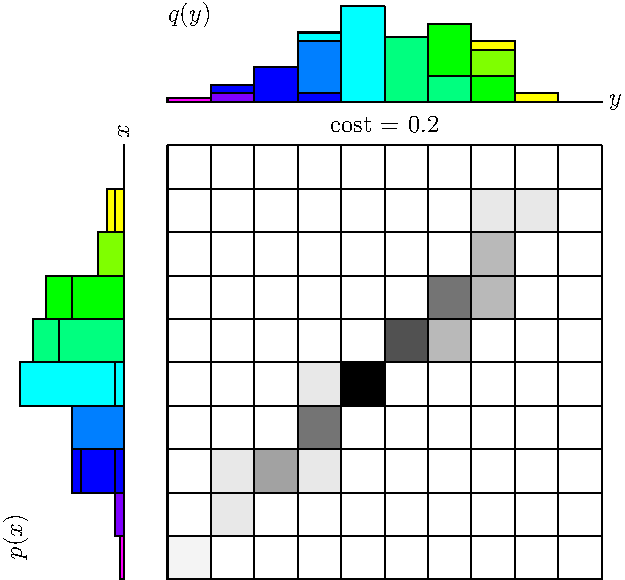
\includegraphics[width=14cm]{transportationCost-5}
\end{minipage}
\end{slide}
\addtocounter{outlineitem}{1}
}

\setcounter{outlineitem}{1}


%%%%%%%%%%%%%%%%%%%%%%% Next Slide %%%%%%%%%%%%%%%%%%%%%%%
\Outline % Comparing Distributions
%%%%%%%%%%%%%%%%%%%%%%% Next Slide %%%%%%%%%%%%%%%%%%%%%%%

\begin{slide}
\section{Measuring Distances Between Distributions}

\begin{PauseHighLight}
  \begin{itemize}
  \item In many machine learning tasks we want to minimise the
    distance between two probability distributions (e.g.\ make a
    generative model's samples look like the data)\pause
  \item This requires that we can measure distances between
    probability distributions\pause
  \item One prominent measure is the Kullback-Leibler or KL divergence
    \begin{align*}
      \mathrm{KL}(p\|q) = \int p(\bm{x}) \,
      \logg{\frac{p(\bm{x})}{q(\bm{x})}} \, \dd \bm{x}\pause
    \end{align*}
  \item This is very commonly used in ML (e.g. VAEs, Variational
    Approximation)\pause
  \end{itemize}
\end{PauseHighLight}

\end{slide}

%%%%%%%%%%%%%%%%%%%%%%% Next Slide %%%%%%%%%%%%%%%%%%%%%%%

\begin{slide}
\section[-2]{Trouble with KL}

\begin{PauseHighLight}
  \begin{itemize}
  \item KL-divergences are non-negative quantities that are minimised
    when the two probability distributions are the same\pause
  \item They are not distances (they aren't symmetric and they don't
    satisfy the triangular inequality)\pause
  \item
    \begin{rightImage}{divergentKL}
      We don't really care about this, but what we do care about is
    that if $q(\bm{x})=0$ when $p(\bm{x})\neq 0$ then
    $\logg{\frac{p(\bm{x})}{q(\bm{x})}}$ diverges\pause
    \end{rightImage}
  \item We can therefore have distributions that seem very similar but
    their KL-divergence is huge (or infinite)\pause
  \end{itemize}
\end{PauseHighLight}

\end{slide}

%%%%%%%%%%%%%%%%%%%%%%% Next Slide %%%%%%%%%%%%%%%%%%%%%%%

\begin{slide}
\section[-1]{Wasserstein Distance}

\begin{PauseHighLight}
  \begin{itemize}
  \item A more benign measure of the differences between two
    probability distributions is the \emph{Wasserstein} or \emph{Earth
      Mover's} distance\pause
  \item
    \begin{rightImage}{divergentKL}
    This is a true distance, but more importantly, it
    measures distance in a very natural way so that distributions that
    are close have a small Wasserstein distance\pause
    \end{rightImage}
  \item This may seem contrived, but images (e.g.\ $128\times128\times3$
    arrays of pixel values) lie close to a thin manifold, so two
    distributions of images can be close without overlapping: then the
    KL-divergence is useless but the Wasserstein distance is not\pause
  \end{itemize}
\end{PauseHighLight}

\end{slide}

%%%%%%%%%%%%%%%%%%%%%%% Next Slide %%%%%%%%%%%%%%%%%%%%%%%

\begin{slide}
\section[-2]{High Probability Manifold}

\begin{center}
  \makebox(100,170)[c]{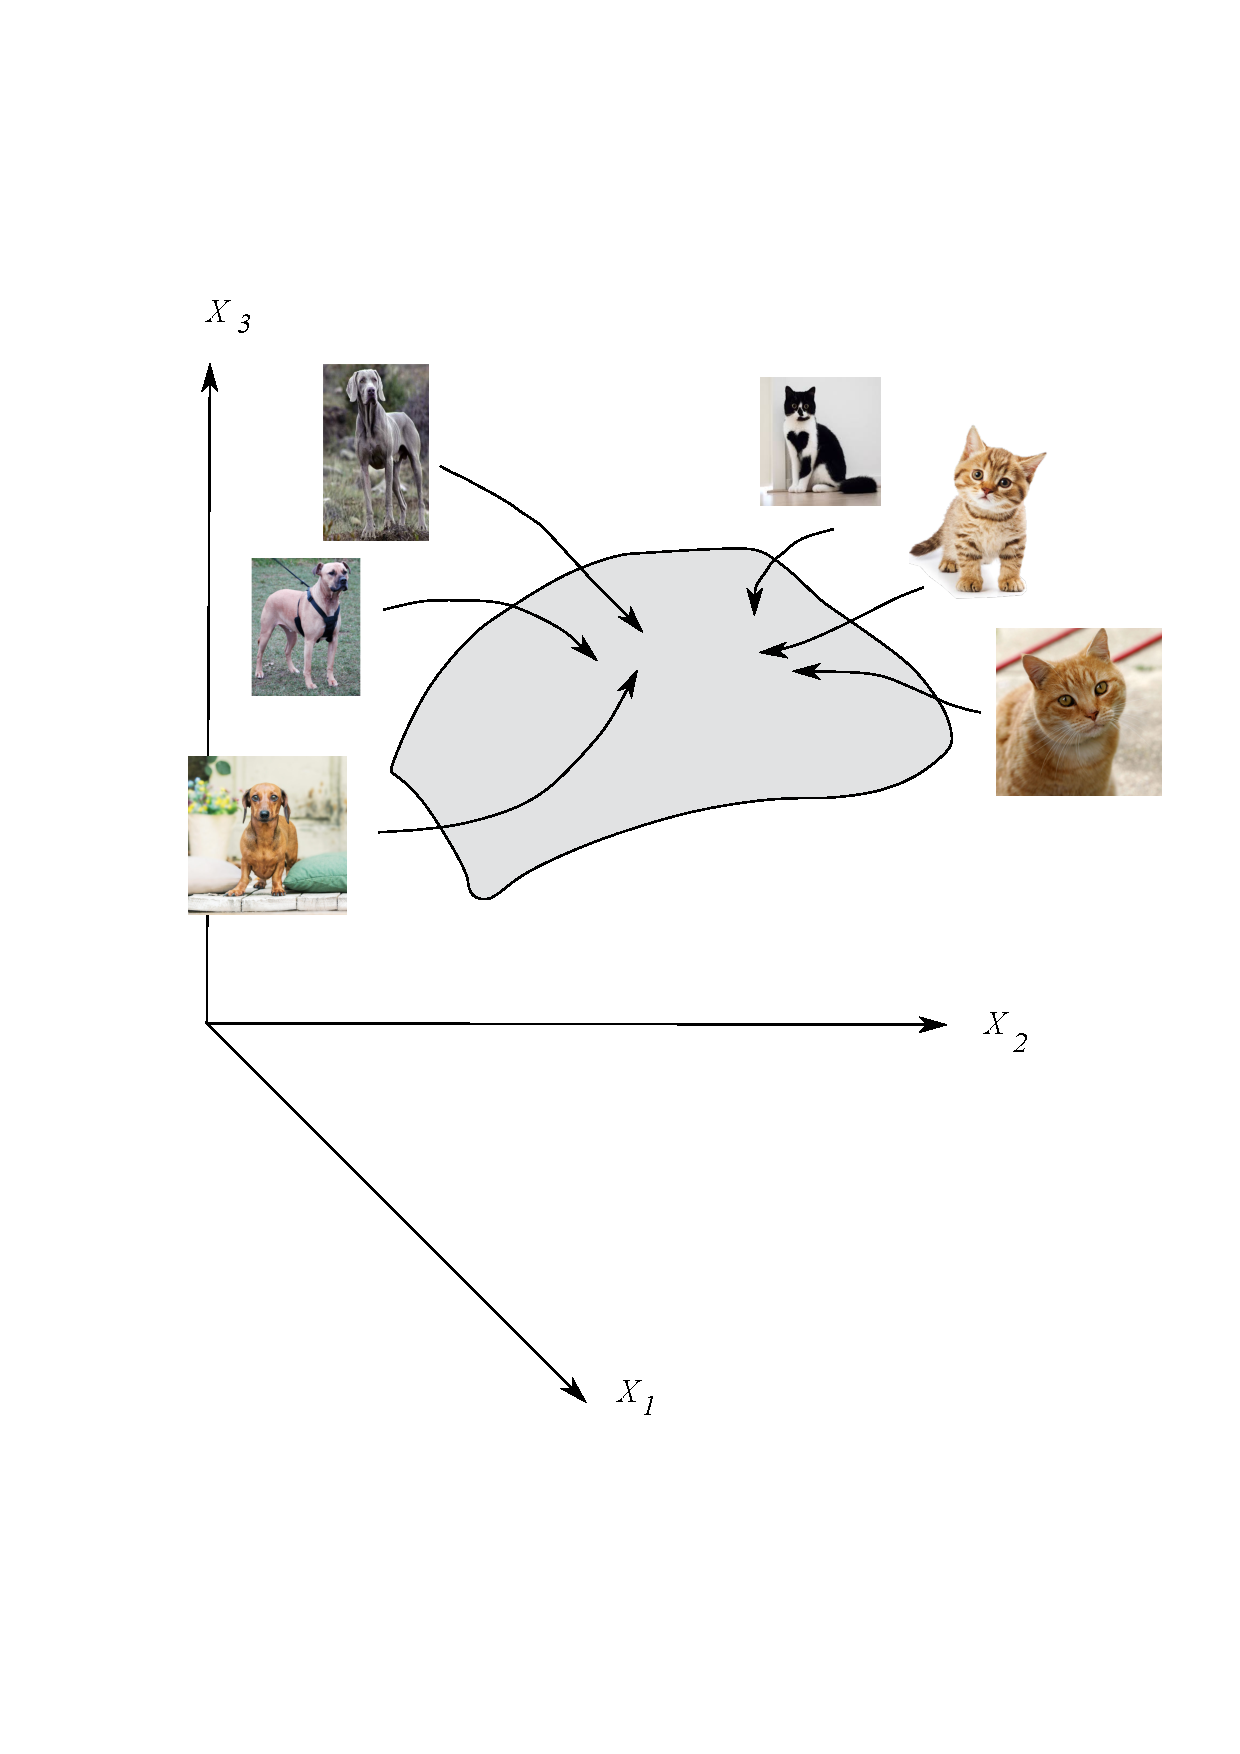
\includegraphics[width=0.7\linewidth]{manifold}}
\end{center}
\end{slide}

%%%%%%%%%%%%%%%%%%%%%%% Next Slide %%%%%%%%%%%%%%%%%%%%%%%
\Outline % Optimal Transport
%%%%%%%%%%%%%%%%%%%%%%% Next Slide %%%%%%%%%%%%%%%%%%%%%%%

\begin{slide}
\section{Transportation Policy}

\begin{PauseHighLight}
  \begin{itemize}
  \item But how do we formalise the Wasserstein distance?\pause
  \item A good place to start is to define a transportation policy
    $\gamma(\bm{x},\bm{y})$ with
    \begin{align*}
      \int \gamma(\bm{x},\bm{y}) \, \dd \bm{y} &= p(\bm{x}) &
      \int \gamma(\bm{x},\bm{y}) \, \dd \bm{x} &= q(\bm{y})\pause
    \end{align*}
  \item This looks like a joint probability distribution, but we
    interpret $\gamma(\bm{x},\bm{y})$ as the amount of probability
    mass/density that we transfer from $p(\bm{x})$ to $q(\bm{y})$\pause
  \end{itemize}
\end{PauseHighLight}

\end{slide}

%%%%%%%%%%%%%%%%%%%%%%% Next Slide %%%%%%%%%%%%%%%%%%%%%%%

\begin{slide}
\section[-2]{Transportation Policy}

\pb
\pause\pauselevel{=1}
\begin{center}
  \multipdf[width=0.65\linewidth]{transportationPolicy}\pause
\end{center}
\end{slide}

%%%%%%%%%%%%%%%%%%%%%%% Next Slide %%%%%%%%%%%%%%%%%%%%%%%

\begin{slide}
\section{The Cost of Transport}

\begin{PauseHighLight}
  \begin{itemize}
  \item We want the transportation policy that minimises the total work:
    the probability mass moved times the distance it is moved\pause
  \item Let $d(\bm{x},\bm{y})=\|\bm{x}-\bm{y}\|$ be a distance measure
    then the cost of a transportation policy is
    \begin{align*}
      C(\gamma) = \int \int d(\bm{x},\bm{y})\,\gamma(\bm{x},\bm{y}) \,
      \dd\bm{x}\,\dd\bm{y}\pause = \av[\gamma]{d(\bm{x},\bm{y})}
    \end{align*}
    where we interpret $\gamma(\bm{x},\bm{y})$ as a probability
    distribution\pauseb
  \item Usually we take $d(\bm{x},\bm{y})$ to be the Euclidean
    distance, but we can choose any distance\pause
  \end{itemize}
\end{PauseHighLight}

\end{slide}

%%%%%%%%%%%%%%%%%%%%%%% Next Slide %%%%%%%%%%%%%%%%%%%%%%%

\begin{slide}
\section[-2]{Transportation Cost}

\pb
\pause\pauselevel{=1}
\begin{center}
  \multipdf[width=0.65\linewidth]{transportationCost}\pause
\end{center}
\end{slide}

%%%%%%%%%%%%%%%%%%%%%%% Next Slide %%%%%%%%%%%%%%%%%%%%%%%

\begin{slide}
\section{The Wasserstein Distance}

\begin{PauseHighLight}
  \begin{itemize}
  \item The Wasserstein distance $W(p,q)$ between two probability
    distributions is defined as
    \begin{align*}
      W(p,q) = \min_{\gamma \in \Lambda(p,q)}
      \av[\gamma]{d(\bm{x},\bm{y})}\pause
    \end{align*}
  \item Where $\Lambda(p,q)$ is the set of joint distributions
    $\gamma(\bm{x},\bm{y})$ such that
    \begin{align*}
      \int \gamma(\bm{x},\bm{y}) \, \dd \bm{y} &= p(\bm{x}) &
      \int \gamma(\bm{x},\bm{y}) \, \dd \bm{x} &= q(\bm{y})\pause
    \end{align*}
  \item With cost $d^k$ we get $W_k(p,q) = \bigl(\min_\gamma
    \av[\gamma]{d(\bm{x},\bm{y})^k}\bigr)^{1/k}$; here we use $W = W_1$\pause
  \end{itemize}
\end{PauseHighLight}

\end{slide}

%%%%%%%%%%%%%%%%%%%%%%% Next Slide %%%%%%%%%%%%%%%%%%%%%%%

\begin{slide}
\section[-2]{One Dimension}

\begin{PauseHighLight}
  \begin{itemize}
  \item In one dimension the Wasserstein distance has a closed form in
    terms of the cumulative distribution functions $F_p$ and $F_q$
    \begin{align*}
      W(p,q) = \int_{-\infty}^{\infty} \bigl|F_p(x) - F_q(x)\bigr|\,\dd x\pause
    \end{align*}
    the area between the two curves\pause
  \item For two samples of the same size: sort both and match them in
    order
    \begin{align*}
      W = \frac{1}{n}\sum_{i=1}^n \bigl|x_{(i)} - y_{(i)}\bigr|\pause
    \end{align*}
  \item In higher dimensions there is no such shortcut: we have to
    solve the optimisation\pause
  \end{itemize}
\end{PauseHighLight}

\end{slide}

%%%%%%%%%%%%%%%%%%%%%%% Next Slide %%%%%%%%%%%%%%%%%%%%%%%
\Outline % Duality
%%%%%%%%%%%%%%%%%%%%%%% Next Slide %%%%%%%%%%%%%%%%%%%%%%%

\begin{slide}
\section[-1]{Computing the Wasserstein Distance}

\begin{PauseHighLight}
  \begin{itemize}
  \item To compute the Wasserstein distance we have to solve a
    minimisation task!\pause
  \item This looks nasty, but it is a (continuous) linear programme,
    like those in the constrained-optimisation lecture\pause
  \item Suppose $p$ and $q$ were discrete distributions (i.e. $\bm{x}$
    and $\bm{y}$ only take discrete points)\pause
  \item Then we could treat each value of $\gamma(\bm{x},\bm{y})$ as
    an element of a vector $\bm{\gamma}$ and each value of
    $d(\bm{x},\bm{y})$ as an element of a vector $\bm{D}$\pause
  \item Our objective is to choose $\bm{\gamma}$ to minimise
    $\bm{D}^\tr\bm{\gamma}$\pause
  \end{itemize}
\end{PauseHighLight}

\end{slide}

%%%%%%%%%%%%%%%%%%%%%%% Next Slide %%%%%%%%%%%%%%%%%%%%%%%

\begin{slide}
\section[-3]{Constraints}
  
\begin{PauseHighLight}
  {\small
\begin{align*}
  \sum_j \gamma(\bm{x}_i,\bm{y}_j) &= p(\bm{x}_i) &
 \sum_i \gamma(\bm{x}_i,\bm{y}_j) &= q(\bm{y}_j)
\end{align*}}
\begin{center}
  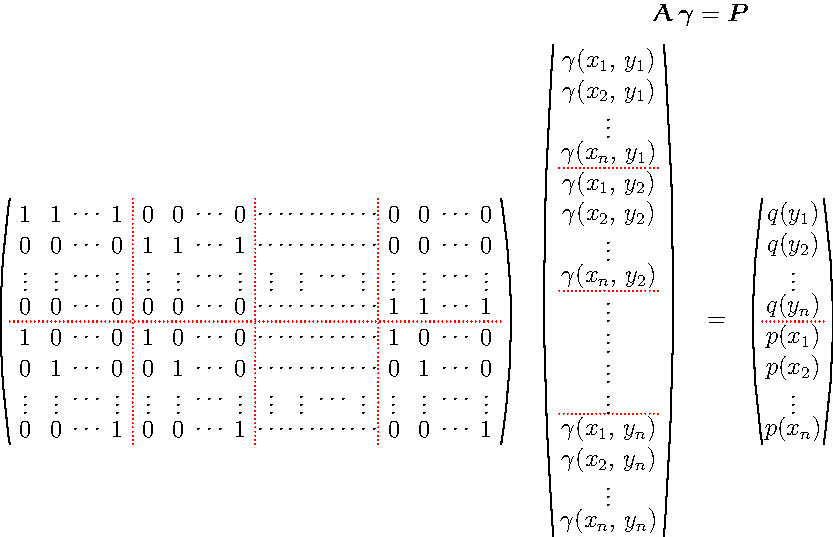
\includegraphics[width=0.8\linewidth]{Amat}\pause
\end{center}
\end{PauseHighLight}

\end{slide}

%%%%%%%%%%%%%%%%%%%%%%% Next Slide %%%%%%%%%%%%%%%%%%%%%%%

\begin{slide}
  \section[-1]{The Dual Problem}


\begin{PauseHighLight}
  \begin{itemize}\footnotesize
  \item With Lagrange multipliers $\alpha(\bm{x}_i)$ and $\beta(\bm{y}_j)$ for
    the two sets of constraints
    \begin{align*}
      \mathcal{L} = \sum_{i,j} d(\bm{x}_i,\bm{y}_j)
      \gamma(\bm{x}_i,\bm{y}_j)
      &- \sum_i \alpha(\bm{x}_i) \left( \sum_j \gamma(\bm{x}_i,\bm{y}_j) -p(\bm{x}_i)\right)\\
      &- \sum_j \beta(\bm{y}_j) \left( \sum_i \gamma(\bm{x}_i,\bm{y}_j) -q(\bm{y}_j)\right)
    \end{align*}
    subject to $\gamma(\bm{x}_i,\bm{y}_j)\geq 0$\pauseb
  \item Rearranging
    \begin{align*}
      \mathcal{L} = \sum_i \alpha(\bm{x}_i)\,p(\bm{x}_i) + \sum_j \beta(\bm{y}_j)\,q(\bm{y}_j)
      -\sum_{i,j} \gamma(\bm{x}_i,\bm{y}_j)\left( \alpha(\bm{x}_i) + \beta(\bm{y}_j) -
      d(\bm{x}_i,\bm{y}_j)\right)\pause
    \end{align*}
  \item This is equivalent to maximising $\sum_i \alpha(\bm{x}_i)\,p(\bm{x}_i) +
    \sum_j \beta(\bm{y}_j)\,q(\bm{y}_j)$, subject to
    \begin{align*}
      \forall i,j \quad \alpha(\bm{x}_i) + \beta(\bm{y}_j) \leq d(\bm{x}_i,\bm{y}_j)\pause
    \end{align*}
  \item For continuous distributions sums become integrals and
    $\alpha(\bm{x})$, $\beta(\bm{y})$ become functions\pause
  \end{itemize}
\end{PauseHighLight}

\end{slide}

%%%%%%%%%%%%%%%%%%%%%%% Next Slide %%%%%%%%%%%%%%%%%%%%%%%

\begin{slide}
\section[-1]{Dual Form Constraint}

\begin{PauseHighLight}\squeeze
  \begin{itemize}
  \item We need $\alpha(\bm{x}) + \beta(\bm{y}) \leq d(\bm{x},\bm{y})$
    for all $\bm{x}$, $\bm{y}$, and want $\beta$ as large as
    possible\pause
  \item Taking $\bm{x}=\bm{y}$ (where $d(\bm{y},\bm{y})=0$) gives
    $\beta(\bm{y}) \leq -\alpha(\bm{y})$;\pause{} so $-\alpha$ is the
    largest $\beta$ could possibly be\pause
  \item Try that largest value, $\beta = -\alpha$: the constraint becomes
    \begin{align*}
      \alpha(\bm{x}) - \alpha(\bm{y}) \leq d(\bm{x},\bm{y})
      \quad\text{for all } \bm{x},\bm{y}\pause
    \end{align*}
  \item For any $\alpha$ that satisfies this, $\beta=-\alpha$ is allowed
    and cannot be beaten\pause
  \item Restricting to such $\alpha$ loses nothing (the
    \emph{Kantorovich--Rubinstein} theorem; see the notes)\pause
  \end{itemize}
\end{PauseHighLight}

\end{slide}

%%%%%%%%%%%%%%%%%%%%%%% Next Slide %%%%%%%%%%%%%%%%%%%%%%%

\begin{slide}
\section[-1]{Kantorovich--Rubinstein Duality}

\begin{PauseHighLight}
  \begin{itemize}
  \item Putting this together
    \begin{align*}
      W(p,q) &= \max_{\alpha} \int \alpha(\bm{x})\,\bigl(p(\bm{x})-q(\bm{x})\bigr)\,\dd\bm{x}\\
      &= \max_{\alpha}\Bigl(\av[p]{\alpha(\bm{X})} - \av[q]{\alpha(\bm{X})}\Bigr)\pause
    \end{align*}
  \item where the maximum is over functions with
    \begin{align*}
      \alpha(\bm{x}) - \alpha(\bm{y}) \leq d(\bm{x},\bm{y}) = \|\bm{x}-\bm{y}\|\pause
    \end{align*}
    that is, $\alpha$ is \emph{1-Lipschitz} (Lipschitz-1)\pause
  \item Instead of the huge object $\gamma(\bm{x},\bm{y})$ we now need one
    function $\alpha(\bm{x})$\pause, and the expectations can be estimated
    from samples\pause
  \end{itemize}
\end{PauseHighLight}

\end{slide}

%%%%%%%%%%%%%%%%%%%%%%% Next Slide %%%%%%%%%%%%%%%%%%%%%%%

\begin{slide}
\section[-2]{Lipschitz-1 Functions}

\begin{PauseHighLight}
  \begin{itemize}
  \item We note for a Lipschitz-1 function and any unit vector $\bm{u}$
    \begin{align*}
      \bm{u}^\tr\grad \alpha(\bm{x}) = \lim_{\epsilon \rightarrow 0}
      \frac{\alpha(\bm{x}+\epsilon \,\bm{u})-\alpha(\bm{x})}{\epsilon}
      \pause
      \leq  \frac{\epsilon\len{\bm{u}}}{\epsilon} \pauseb = \frac{\epsilon}{\epsilon} = 1 \pauseb
    \end{align*}
  \item That is, at every point the gradient in every direction is at
    most 1\pause{} (since the gradient defines the direction of greatest
    increase it is both necessary and sufficient for $\|\grad
    \alpha(\bm{x})\|\leq1$ everywhere)\pauseb
  \end{itemize}
  \begin{center}
    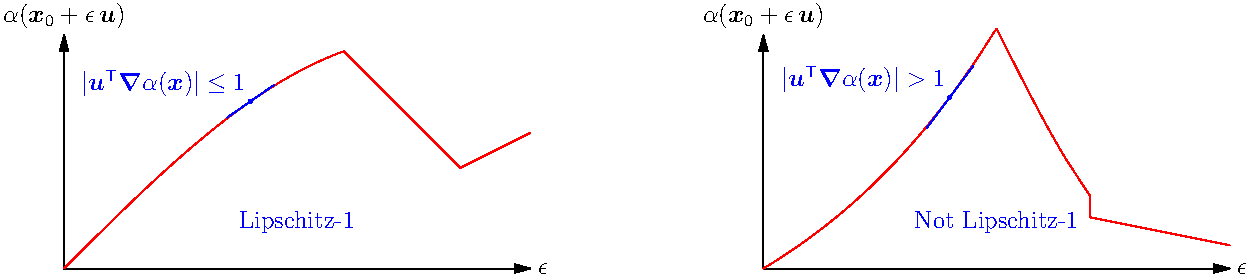
\includegraphics[width=\linewidth]{Lipschitz1}\pause
  \end{center}
\end{PauseHighLight}
  

\end{slide}

%%%%%%%%%%%%%%%%%%%%%%% Next Slide %%%%%%%%%%%%%%%%%%%%%%%
\Outline % Applications
%%%%%%%%%%%%%%%%%%%%%%% Next Slide %%%%%%%%%%%%%%%%%%%%%%%

\begin{slide}
\section{How GANs Work}

\pb\pause\pauselevel{=1}
\begin{center}
  \multipdf[width=\linewidth]{gan}\pause
\end{center}
\end{slide}

%%%%%%%%%%%%%%%%%%%%%%% Next Slide %%%%%%%%%%%%%%%%%%%%%%%

\begin{slide}
\section[-1]{Wasserstein GANs}

\begin{PauseHighLight}
  \begin{itemize}\squeeze
  \item A GAN has a \emph{generator} $G(\bm{z},\bm{w}_G)$ that turns
    noise $\bm{z}\sim\mathcal{N}(\bm{0},\mat{I})$ into images, and a
    \emph{discriminator} trained to tell them from real images\pause
  \item GANs are hard to train: a discriminator that is too good gives
    the generator no useful gradient\pause
  \item A Wasserstein GAN instead trains the generator to minimise $W$
    between the data distribution $p$ and the generator's distribution $q$
    \begin{align*}
      \min_{\bm{w}_G}\,\max_{\alpha}\Bigl(\av[p]{\alpha(\bm{x})} -
      \av[\bm{z}]{\alpha(G(\bm{z},\bm{w}_G))}\Bigr)\pause
    \end{align*}
  \item The \emph{critic} $\alpha$ is a second network in place of the
    discriminator; it still gives a gradient when the distributions do
    not overlap\pause
  \end{itemize}
\end{PauseHighLight}

\end{slide}

%%%%%%%%%%%%%%%%%%%%%%% Next Slide %%%%%%%%%%%%%%%%%%%%%%%

\begin{slide}
\section[-1]{The Critic}

\begin{PauseHighLight}
  \begin{itemize}
  \item Estimate the expectations from a minibatch $\mathcal{B}$ of real
    images and $n$ generated ones
    \begin{align*}
      C = \frac{1}{|\mathcal{B}|} \sum_{\bm{x}\in\mathcal{B}} \alpha(\bm{x},\bm{w}_\alpha) -
      \frac{1}{n} \sum_{i=1}^n \alpha(G(\bm{z}_i,\bm{w}_G),\bm{w}_\alpha)\pause
    \end{align*}
  \item The critic's weights $\bm{w}_\alpha$ are trained to maximise $C$;
    the generator's weights $\bm{w}_G$ to minimise it\pause
  \item The critic should be 1-Lipschitz, which in practice is only
    roughly enforced: by clipping the weights (the original WGAN),
    penalising $\|\grad\alpha\|$ away from 1, or scaling each weight
    matrix to spectral norm 1\pause
  \end{itemize}
\end{PauseHighLight}

\end{slide}

%%%%%%%%%%%%%%%%%%%%%%% Next Slide %%%%%%%%%%%%%%%%%%%%%%%

\begin{slide}
\section{Wasserstein GANs}

\pb\pause\pauselevel{=1}
\begin{center}
  \multipdf[width=\linewidth]{wgan}\pause
\end{center}
\end{slide}

%%%%%%%%%%%%%%%%%%%%%%% Next Slide %%%%%%%%%%%%%%%%%%%%%%%

\begin{slide}
\section[-2]{Entropic Regularisation}

\begin{PauseHighLight}
  \begin{itemize}
  \item Solving the linear programme for $n$ points costs roughly
    $O(n^3)$: too slow for large problems\pause
  \item Cuturi (2013) added an entropy term, with $\epsilon>0$
    \begin{align*}
      \min_{\gamma}\; \sum_{i,j} d_{ij}\,\gamma_{ij} + \epsilon\sum_{i,j}
      \gamma_{ij}\log\gamma_{ij}
    \end{align*}
    with the same constraints\pause
  \item The optimisation is given by: $\displaystyle
    \max_{\bm{\alpha},\bm{\beta}} \; \min_{\gamma}\;
    \mathcal{L}(\gamma, \bm{\alpha}, \bm{\beta})$
    {\small
    \begin{align*}
      \mathcal{L} = \sum_{i,j} d_{ij}\,\gamma_{ij} + \epsilon\sum_{i,j}
      \gamma_{ij}\log\gamma_{ij} - \sum_i \alpha_i \bra{\sum_j
      \gamma_{ij} - p_i}  - \sum_j \beta_j \bra{\sum_i
      \gamma_{ij} - q_j}\pause
    \end{align*}}
  \end{itemize}
\end{PauseHighLight}

\end{slide}

%%%%%%%%%%%%%%%%%%%%%%% Next Slide %%%%%%%%%%%%%%%%%%%%%%%

\begin{slide}
\section[-2]{Solving the Primal Problem}

\begin{PauseHighLight}
  \begin{itemize}
  \item Using
    {\small
    \begin{align*}
      \mathcal{L} = \sum_{i,j} d_{ij}\,\gamma_{ij} + \epsilon\sum_{i,j}
      \gamma_{ij}\log\gamma_{ij} - \sum_i \alpha_i \bra{\sum_j
      \gamma_{ij} - p_i}  - \sum_j \beta_j \bra{\sum_i
      \gamma_{ij} - q_j}\pause
    \end{align*}}
  \item Setting the derivative of the Lagrangian to zero gives
    \begin{align*}
      \gamma_{ij} = \e{(\alpha_i - d_{ij} + \beta_j)/\epsilon - 1}
       = u_i\,K_{ij}\,v_j
    \end{align*}
    where $u_i=  \e{\alpha_i/\epsilon-1}$, $v_j=\e{\beta_j/\epsilon}$
    and $K_{ij} = \e{-d_{ij}/\epsilon}$\pause
  \item We have to choose $u_i$ and $v_j$ (equivalently the Lagrange
    multipliers) so that
    \begin{align*}
      \sum_j u_i\,K_{ij}\,v_j &= p_i & \sum_i u_i\,K_{ij}\,v_j &= q_j\pause
    \end{align*}
  \end{itemize}
\end{PauseHighLight}

\end{slide}


%%%%%%%%%%%%%%%%%%%%%%% Next Slide %%%%%%%%%%%%%%%%%%%%%%%

\begin{slide}
\section[-1]{The Sinkhorn Algorithm}

\begin{PauseHighLight}
  \begin{itemize}\squeeze
  \item Choose $\bm{u}$ and $\bm{v}$ so the row and column sums are $\bm{p}$
    and $\bm{q}$: alternately rescale ($\oslash$ is element-by-element
    division)
    \begin{align*}
      \bm{v} \leftarrow \bm{q}\oslash(\mat{K}^\tr\bm{u}), \qquad
      \bm{u} \leftarrow \bm{p}\oslash(\mat{K}\bm{v})\pause
    \end{align*}
  \item This is Sinkhorn's matrix-scaling algorithm: each step is
    two matrix--vector products\pause
  \item Fast on GPUs and differentiable, so it can sit inside a loss\pause
  \item As $\epsilon\to0$ we recover the exact transport cost; larger
    $\epsilon$ is faster but blurs the plan\pause
  \item This is how optimal transport is mostly computed in ML today\pause
  \end{itemize}
\end{PauseHighLight}

\end{slide}

%%%%%%%%%%%%%%%%%%%%%%% Next Slide %%%%%%%%%%%%%%%%%%%%%%%

\begin{slide}
\section[-2]{Sinkhorn in Action}

\pb
\pause\pauselevel{=1}
\begin{center}
  \multipdf[width=0.55\linewidth]{sinkhorn}\pause
\end{center}
\end{slide}

%%%%%%%%%%%%%%%%%%%%%%% Next Slide %%%%%%%%%%%%%%%%%%%%%%%

\begin{slide}
\section[-2]{Evaluating Generative Models: FID}

\begin{PauseHighLight}
  \begin{itemize}
  \item For Gaussians, $W_2$ has a closed form
    \begin{align*}
      W_2^2 = \|\bm{\mu}_1-\bm{\mu}_2\|^2 + \mathrm{Tr}\!\left(\mat{\Sigma}_1 +
      \mat{\Sigma}_2 - 2\bigl(\mat{\Sigma}_1\mat{\Sigma}_2\bigr)^{1/2}\right)\pause
    \end{align*}
    (in one dimension $(\mu_1-\mu_2)^2 + (\sigma_1-\sigma_2)^2$)\pause
  \item The \emph{Fr\'echet Inception Distance} (Heusel et al., 2017) fits
    Gaussians to a pretrained network's features of real and of
    generated images, and reports this distance\pause
  \item It is the standard score for image generators, GANs and
    diffusion models alike (lower is better)\pause
  \item Caveat: it only compares means and covariances of the
    features\pause
  \end{itemize}
\end{PauseHighLight}

\end{slide}

%%%%%%%%%%%%%%%%%%%%%%% Next Slide %%%%%%%%%%%%%%%%%%%%%%%

\begin{slide}
\section[-1]{Lessons}

\begin{PauseHighLight}
  \begin{itemize}
  \item The Wasserstein distance compares distributions by how far
    probability mass must move, so it behaves well when they do not
    overlap\pause
  \item Computing it is a linear programme, whose dual is a maximum
    over 1-Lipschitz functions\pause
  \item That dual turned GANs into Wasserstein GANs: an elegant piece of
    theory\pause
  \item In practice optimal transport is computed with Sinkhorn, and the
    $W_2$ distance between Gaussians is the FID used to evaluate
    generative models\pause
  \end{itemize}
\end{PauseHighLight}

\end{slide}

\end{document}
